%
\subsection{Detection \& Estimation}
\begin{problem}
Let $X \in \cbrak{1,-1}$.  Generate $X$ such that the numbers 1 and -1 appear with equal probability.  This is a random variable formulation of the coin tossing experiment.
\end{problem}
\solution  The following script generates the numbers 1 and -1 with 
equal probability.
\lstinputlisting{./chapter2/codes/2.1.py}
%
\begin{problem}
Verify that the script in the previous problem generates equiprobable symbols.
\end{problem}
\begin{problem}
Suppose $X \in \cbrak{1,-1}$ and 
%
\begin{equation}
Y = AX + N
\end{equation}
%
where $N \sim \gauss{0}{1}$ and $A = 4$.  Plot $Y$.
\end{problem}
\solution The following code yields Fig. \ref{ch2_bpsk_sim}
\lstinputlisting{./chapter2/codes/2.3.py}
%
\begin{figure}
\centering
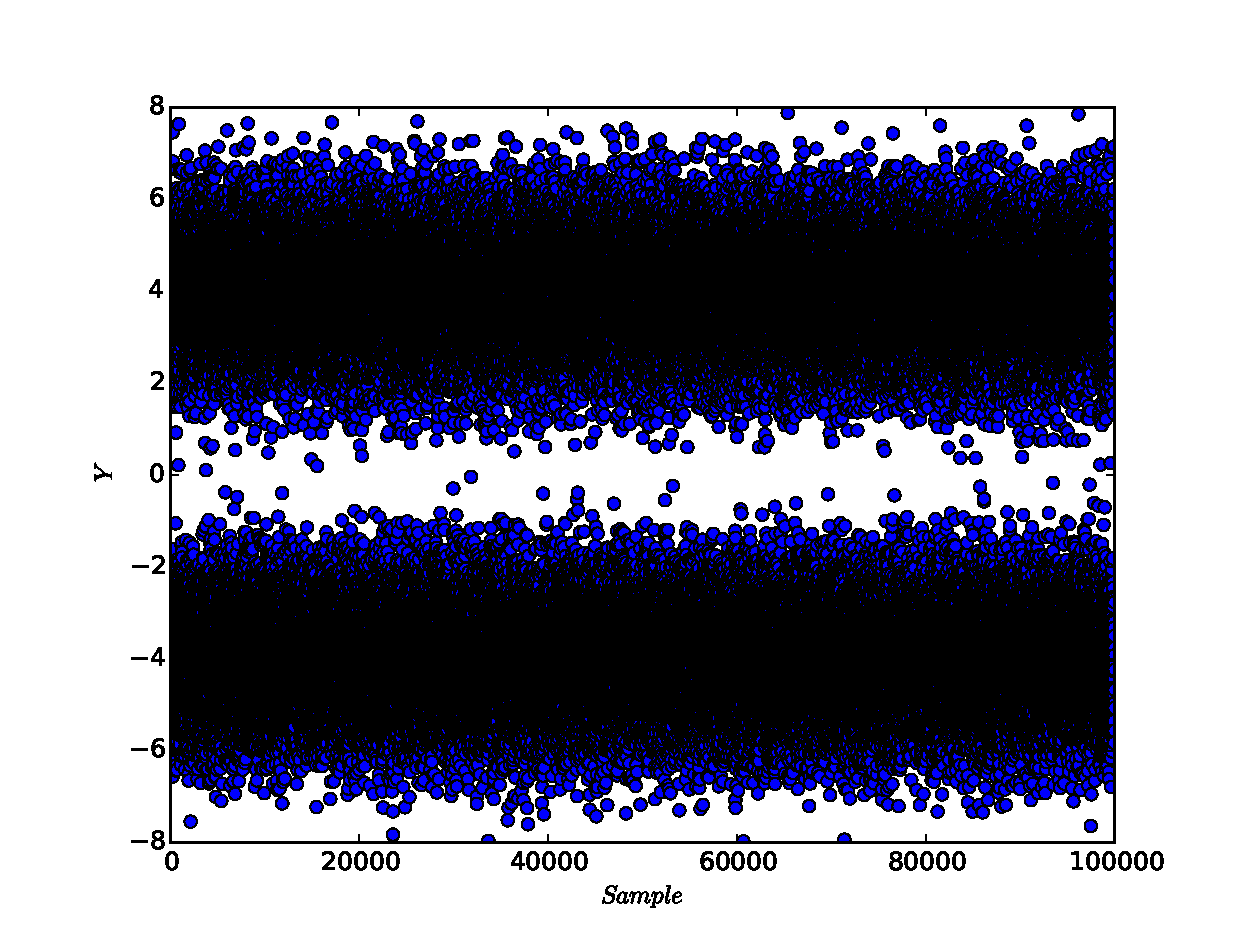
\includegraphics[width=\columnwidth]{./chapter2/figs/ch2_bpsk_sim}
\caption{Plot of $Y$}
\label{ch2_bpsk_sim}
\end{figure}
%
\begin{problem}
Given $Y$ in the previous problem, how would you decide whether $X$ is 1
or -1.
\end{problem}
%
\begin{problem}
Suppose $X=1$ and $\hat{X}$ is what you detected.  Find $\pr{\hat{X}=-1/X=1}$.
\end{problem}
%
\begin{problem}
Plot  $\pr{\hat{X}=-1/X=1}$ with respect to $A$.
\end{problem}
%
\begin{problem}
For $X \sim \mathcal{N}\brak{0,1}$, the $Q$-function is defined as
\begin{equation}
Q(x) = \pr{X > x}, \quad x > 0
\end{equation}
Express $\pr{\hat{X}=-1/X=1}$ in terms of the $Q$-function. Plot this expression with respect to $A$ and compare with the result obtained through simulation.
\end{problem}
%
\begin{problem}
The signal to noise ratio of the above system is defined as 
\begin{equation}
SNR = \frac{A^2}{\mean{N^2}}
\end{equation}
Plot the thoeretical and simulated values of $\pr{\hat{X}=-1/X=1}$ for the SNR ranging from 0 to 10 dB.
\end{problem}
%
\begin{problem}
Now consider a threshold $\lambda > 0$ and find the average probability of error. Plot this with respect to $\lambda$.
\end{problem}
%
\begin{problem}
From the graph in the previous problem, find the optimum threshold so that the probability of error is minimum.
\end{problem}
%
\subsection{The MAP criterion}
%
A Gaussian random variable $Y\sim\gauss{\mu}{\sigma^2}$ has the pdf
%
\begin{equation}
p_{Y}(x) = \frac{1}{\sqrt{2\pi}\sigma}e^{-\brak{x-\mu}^2/2\sigma^2} - \infty < x < \infty
\end{equation}
%
\begin{problem}
Plot
\begin{equation}
p_{Y}(Y|X=1) \text{ and } p_{Y}(Y|X=-1)
\end{equation}
in the same graph with respect to $A$.
\end{problem}

\begin{problem}
Graphically obtain the decision resulting from
\begin{equation}
p_{Y}(Y|X=1) \dec{1}{-1} p_{Y}(Y|X=-1)
\end{equation}
Comment.
\end{problem}
